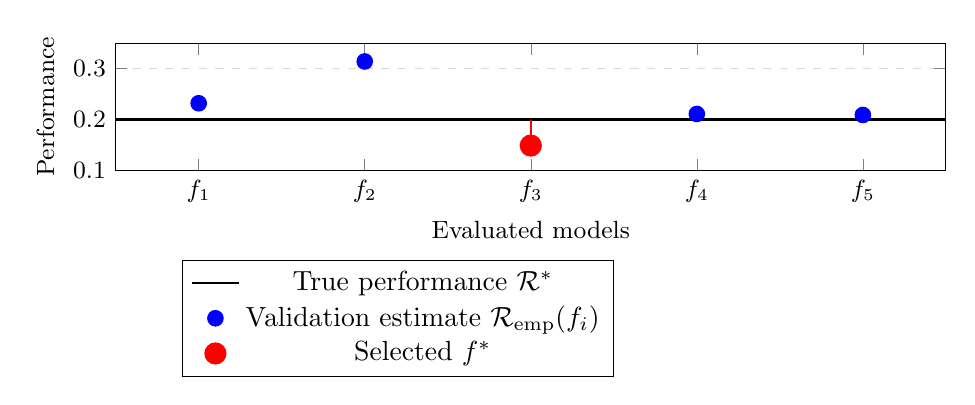
\begin{tikzpicture}
\begin{axis}[
    width=\textwidth,
    height=3.2cm,
    ymin=0.1, ymax=0.35,
    xmin=0.5, xmax=5.5,
    xtick={1,...,5},
    xticklabels={$f_1$,$f_2$,$f_3$,$f_4$,$f_5$},
    ylabel={Performance},
    xlabel={Evaluated models},
    legend style={at={(0.34,-0.7)},anchor=north},
    ymajorgrids=true,
    grid style={dashed,gray!30},
    tick label style={font=\small},
    label style={font=\small},
]

% True performance line
\addplot[
    domain=0.5:5.5,
    samples=2,
    thick,
    black
] {0.2};
\addlegendentry{True performance $\mathcal{R}^\ast$}

% Noisy empirical scores
\addplot[
    only marks,
    mark=*,
    mark size=2.8pt,
    blue
] coordinates {
    (1,0.232)
    (2,0.314)
    (3,0.149)
    (4,0.211)
    (5,0.209)
};
\addlegendentry{Validation estimate $\mathcal{R}_{\mathrm{emp}}(f_i)$}

% Highlight selected model
\addplot[
    only marks,
    mark=*,
    mark size=3.8pt,
    red
] coordinates {(3,0.149)};
\addlegendentry{Selected $f^\ast$}

% Optional vertical line to show optimistic gap
\draw[thick,red] (axis cs:3,0.2) -- (axis cs:3,0.149);

\node[red, align=left, font=\scriptsize] at (axis cs:8.1,0.865)
    {optimistic gap\\caused by noise};

\end{axis}
\end{tikzpicture}